\documentclass[runningheads]{llncs}

\usepackage[T1]{fontenc}
\usepackage[utf8]{inputenc}
\usepackage{amsmath,amssymb}
\usepackage{graphicx}
\usepackage{booktabs}
\usepackage{algorithm}
\usepackage[noend]{algpseudocode}
\usepackage{xspace}
\usepackage[hidelinks]{hyperref}
\hypersetup{pdftitle={Basins, Bridges and Simplification with Morse Sequences},pdfauthor={K\'evin Feltrin}}

% ---------------------------------------------------------------------
% numbers produced by paper/experiments (see paper/README.md)
% generated by paper/experiments/make_numbers.py -- do not edit
\newcommand{\nRWSimages}{830}
\newcommand{\nRWScells}{347\,810}
\newcommand{\nRWSdiff}{0}
\newcommand{\nCancelStacks}{300}
\newcommand{\nCancelPairs}{33\,109}
\newcommand{\nCancelNotFlat}{31\,677}
\newcommand{\nCancelNotFlatPct}{96}
\newcommand{\nMerges}{9\,736}
\newcommand{\nSeqs}{220}
\newcommand{\nSeqCells}{65\,820}
\newcommand{\nStrict}{104}
\newcommand{\runtimeMachine}{Python 3.13.4}
\newcommand{\runtimeMinUs}{44}
\newcommand{\runtimeMaxUs}{121}
\newcommand{\runtimeMaxCells}{1\,046\,529}
\newcommand{\simplN}{64}
\newcommand{\simplNoise}{7}
\newcommand{\simplWells}{6}
\newcommand{\simplMinStart}{662}
\newcommand{\simplHShow}{12}
\newcommand{\simplMinShow}{6}
\newcommand{\simplPlateauLo}{12}
\newcommand{\simplPlateauHi}{16}
\newcommand{\simplMinEnd}{4}
\newcommand{\simplHEnd}{40}
\newcommand{\simplCancel}{658}
\newcommand{\simplSeconds}{176}

% ---------------------------------------------------------------------

\newcommand{\St}{\mathrm{St}}
\newcommand{\Un}{\mathrm{Un}}
\newcommand{\req}{\mathrm{req}}
\newcommand{\lab}{\mathrm{lab}}
\newcommand{\Br}{\mathrm{Br}}
\newcommand{\Fup}{F^{\uparrow}}
\newcommand{\Fdown}{F^{\downarrow}}
\newcommand{\coext}{\widehat{\Upsilon}}
\newcommand{\ext}{\widehat{\Lambda}}
\newcommand{\morseq}{\texttt{morseq}\xspace}

\begin{document}

\title{Basins, Bridges and Simplification with Morse Sequences}
\titlerunning{Basins, Bridges and Simplification with Morse Sequences}
\author{K\'evin Feltrin}
\authorrunning{K. Feltrin}
\institute{ESIEE Paris, Universit\'e Gustave Eiffel, Noisy-le-Grand, France\\
\email{kevin.feltrin@edu.esiee.fr}}

\maketitle

\begin{abstract}
Morse sequences describe the gradient vector fields of discrete Morse theory
by elementary expansions and fillings, so that acyclicity holds by
construction, and their refinement to stacks follows the levels of a
grayscale function. The construction of a gradient field from an image is
thus available with Morse sequences, but the segmentation layer of discrete
Morse theory (stable sets, basins, bridges) and the simplification of
critical pairs are not. We translate this layer, replacing the injective
discrete Morse function of the classical proofs by the insertion order of
the sequence. Stable and unstable sets coincide with their recursive
definitions, whereas the parity-based maps of Morse sequences are strictly
smaller. The basin of a minimum is the unique maximal closure of the
minimum under regular expansions; one scan of the sequence labels all
basins in linear time and serves every level of the stack; the bridges
between basins are exactly the edges of the stable sets of the critical
edges. Cancelling a critical pair
breaks the compatibility of the field with the stack, and we show that it is
restored by two explicit stacks, obtained by filling or cutting one
connected component of a sublevel or superlevel set; cancelling a minimum
with a saddle merges exactly two basins. All statements are implemented in
an open-source library and checked on random fields and images.
\keywords{Discrete Morse theory \and Morse sequences \and Stacks \and
Basins \and Watershed \and Simplification \and Image segmentation}
\end{abstract}

% =====================================================================
\section{Introduction}

Discrete Morse theory~\cite{Forman98,Forman02} replaces the gradient of a
smooth function by an acyclic matching of the cells of a complex. For
grayscale images, Robins, Wood and Sheppard (RWS)~\cite{RWS11} build such a
matching from the pixel values by processing the lower star of each vertex,
and Delgado-Friedrichs, Robins and Sheppard (DFRS)~\cite{DFRS15} read
segmentation objects off its dynamics: stable and unstable sets, basins of
minima, bridges between basins and the Morse skeleton. Critical pairs due
to noise are then removed by cancellation~\cite{Forman98}, which
reverses a gradient path. Related constructions are surveyed
in~\cite{DIMS15}.

Morse sequences~\cite{Ber25a} describe the same fields differently. A
Morse sequence builds a complex by elementary expansions and fillings; its
regular pairs form a gradient vector field, acyclic by construction, and
every gradient vector field arises in this way. Reference and coreference
maps carry homological information along the sequence. On a
\emph{stack}, a monotone function on a complex, an $F$-sequence keeps the
two cells of every pair at the same level and a flooding sequence inserts
the levels in increasing order, as watershed algorithms
do~\cite{Ber25b}. Bertrand and Najman~\cite{BN25} compute such sequences
from vertex maps, with or without ties, and observe that for injective maps
their lower-star algorithm and the one of~\cite{RWS11} have the same core.

The construction stage of the pipeline of~\cite{RWS11,DFRS15} thus has a
counterpart with Morse sequences. The segmentation stage does not: none
of~\cite{Ber25a,Ber25b,BN25} defines stable sets, basins or bridges, and
the stack is always fixed, so that cancellation is not covered either. The
proofs of~\cite{DFRS15} cannot be transcribed as they stand, because they
compare the values of a discrete Morse function assumed to be injective,
which a Morse sequence does not provide and a stack need not be. Watersheds
have been studied in the dual setting where minima are top-dimensional
cells~\cite{BBN23}; here, as in~\cite{DFRS15}, minima are vertices.

\paragraph{Contributions.}
\begin{itemize}
\item The insertion order of a Morse sequence replaces the injective
function (Lemma~\ref{lem:order}). Stable and unstable sets defined by the
existence of paths coincide with the recursive sets of~\cite{DFRS15},
whereas the supports of the extension maps of~\cite{Ber25a}, governed by
parity, are strictly smaller in general; at dimension zero the two notions
agree and the minima partition the vertices (Sect.~\ref{sec:flow}).
\item Prefixes of a sequence and cuts of an $F$-sequence are hermetic, so
stable sets and basins restrict to them. The basin of a minimum is the
unique maximal closure of the minimum under regular expansions, a
constructive form of the definition of~\cite{DFRS15}; one scan labels all
basins in linear time and yields the basins of every cut. The bridges are
exactly the union of the stable sets of the critical edges
(Sect.~\ref{sec:basins}).
\item Cancelling a critical pair breaks the $F$-sequence property in
general. It holds again for two explicit stacks, obtained by raising a
component of a sublevel set or lowering a component of a superlevel set;
for a minimum and a saddle, the first one fills the basin of the minimum up
to the saddle, as in the filtering of minima by
dynamics~\cite{Grimaud92}. Cancelling a minimum with a saddle merges
exactly two basins (Sect.~\ref{sec:simplification}).
\item For images, we make the relation with~\cite{RWS11} precise: a
variant of their algorithm that counts facets instead of faces returns the
same field (Sect.~\ref{sec:lowerstars}).
\item All results are implemented in the open-source library
\morseq~\cite{morseq}, where each statement is an executable test; we
report systematic checks, running times and a simplification example
(Sect.~\ref{sec:experiments}).
\end{itemize}

% =====================================================================
\section{Background}\label{sec:background}

\paragraph{Complexes and fields.}
$K$ is a finite cubical or simplicial complex, identified with its set of
cells ordered by the face relation $\le$. We write $\partial\nu$ for the
set of facets (faces of codimension one) of a cell $\nu$, $K^{(p)}$ for the
set of $p$-cells, and call \emph{subcomplex} a subset closed under faces.
A \emph{discrete vector field} $V$ on $K$ is a set of pairs $(\sigma,\tau)$
with $\sigma\in\partial\tau$, each cell belonging to at most one pair; we
write $V(\sigma)=\tau$. A cell in no pair is \emph{critical}. A
\emph{gradient path} from $\sigma_0$ to $\sigma_r$ is a sequence
$\langle\sigma_0,\tau_0,\sigma_1,\ldots,\tau_{r-1},\sigma_r\rangle$ with
$\tau_i=V(\sigma_i)$ and $\sigma_{i+1}\in\partial\tau_i\setminus\{\sigma_i\}$
($r=0$ is allowed). A \emph{cogradient path} from $\tau_0$ to $\tau_r$ is a
sequence $\langle\tau_0,\sigma_1,\tau_1,\ldots,\sigma_r,\tau_r\rangle$ with
$\sigma_i\in\partial\tau_{i-1}$ and $\tau_i=V(\sigma_i)\ne\tau_{i-1}$. The
field $V$ is a \emph{gradient vector field} if it has no closed non-trivial
gradient path.

\paragraph{Morse sequences~\cite{Ber25a}.}
A \emph{Morse sequence} $W$ is a sequence of subcomplexes
$\emptyset=K_0\subset K_1\subset\cdots\subset K_N=K$ where each
$K_i$ is obtained from $K_{i-1}$ either by a \emph{filling}, which adds one
cell $\kappa_i$, called critical, or by an \emph{expansion}, which adds a
regular pair $\kappa_i=(\sigma,\tau)$ with $\sigma\in\partial\tau$ such that
$(\sigma,\tau)$ is a free pair of $K_i$. The regular pairs form a gradient
vector field $V(W)$, and every gradient vector field is of this
form~\cite[Th.~51]{Ber25a}. We write $t(\nu)=i$ when $\nu$ is inserted at
step $i$, and, for a pair,
$\req(\sigma,\tau)=\partial\sigma\cup(\partial\tau\setminus\{\sigma\})$ for
the cells that the expansion requires. Bertrand associates with $W$ a
\emph{reference map} $\gamma$ and a \emph{coreference map} $\lambda$, linear
over $\mathbb{Z}_2$, and proves that for a critical $p$-cell $\kappa$ and a
$p$-cell $\nu$, $\kappa\in\gamma(\nu)$ iff the number of gradient paths from
$\nu$ to $\kappa$ is odd, and $\kappa\in\lambda(\nu)$ iff the number of
cogradient paths from $\kappa$ to $\nu$ is odd~\cite[Th.~12]{Ber25a}. The
coextension and the extension of $\kappa$ are
$\coext(\kappa)=\{\nu:\kappa\in\gamma(\nu)\}$ and
$\ext(\kappa)=\{\nu:\kappa\in\lambda(\nu)\}$~\cite[Def.~32]{Ber25a}. The
proofs we use rely only on the incidence relation and hold verbatim for
cubical complexes, as noted in~\cite{BN25}.

\paragraph{Stacks~\cite{Ber25b}.}
A \emph{stack} is a map $F:K\to\mathbb{R}$ such that $\sigma\le\tau$ implies
$F(\sigma)\le F(\tau)$; its \emph{cut} at level $\lambda$ is
$F_\lambda=\{\nu:F(\nu)\le\lambda\}$, a subcomplex. The max-extension of a
vertex map $f$, $F(\nu)=\max\{f(v): v\text{ vertex of }\nu\}$, is a stack.
A field is \emph{$F$-flat} if $F(\sigma)=F(\tau)$ for each of its pairs. A
Morse sequence is an \emph{$F$-sequence} if its field is
$F$-flat~\cite[Def.~4]{Ber25b}, and a \emph{flooding sequence} if moreover
$F$ never decreases along it~\cite[Def.~5]{Ber25b}, in which case every cut
is a prefix~\cite[Prop.~7]{Ber25b}. Every $F$-sequence is equivalent to a
flooding sequence~\cite[Th.~4.1]{Ber25b}.

\paragraph{The segmentation layer~\cite{DFRS15}.}
For a critical $p$-cell $\alpha$, DFRS define the stable set $S_K(\alpha)$
as the smallest set of $p$-cells containing $\alpha$ such that
$V(\delta)=\gamma$, $\beta\in\partial\gamma$ and $\beta\in S_K(\alpha)$
imply $\delta\in S_K(\alpha)$; the unstable set $U_K(\alpha)$ is defined
dually. A subcomplex $H$ is \emph{hermetic} if $\sigma\in H$ and
$(\sigma,\tau)\in V$ imply $\tau\in H$; since $H$ is closed under faces, a
pair of $V$ is then entirely inside or entirely outside $H$, and $V_H$
denotes the pairs inside. A collapse is \emph{regular} if its free pairs
belong to $V$. The \emph{basin} of a critical vertex $m$ is the largest
subcomplex that collapses regularly onto $\{m\}$; it is unique
\cite[Lem.~6]{DFRS15}. A \emph{bridge} is a $1$-cell contained in no
basin. The proofs of~\cite{DFRS15} use a discrete Morse function whose
values are pairwise distinct.

Throughout, $W$ is a Morse sequence on $K$ with field $V=V(W)$, and
$\mathcal{M}$ is its set of critical vertices.
Figure~\ref{fig:running} shows the example used in the figures.

\begin{figure}[t]
\centering
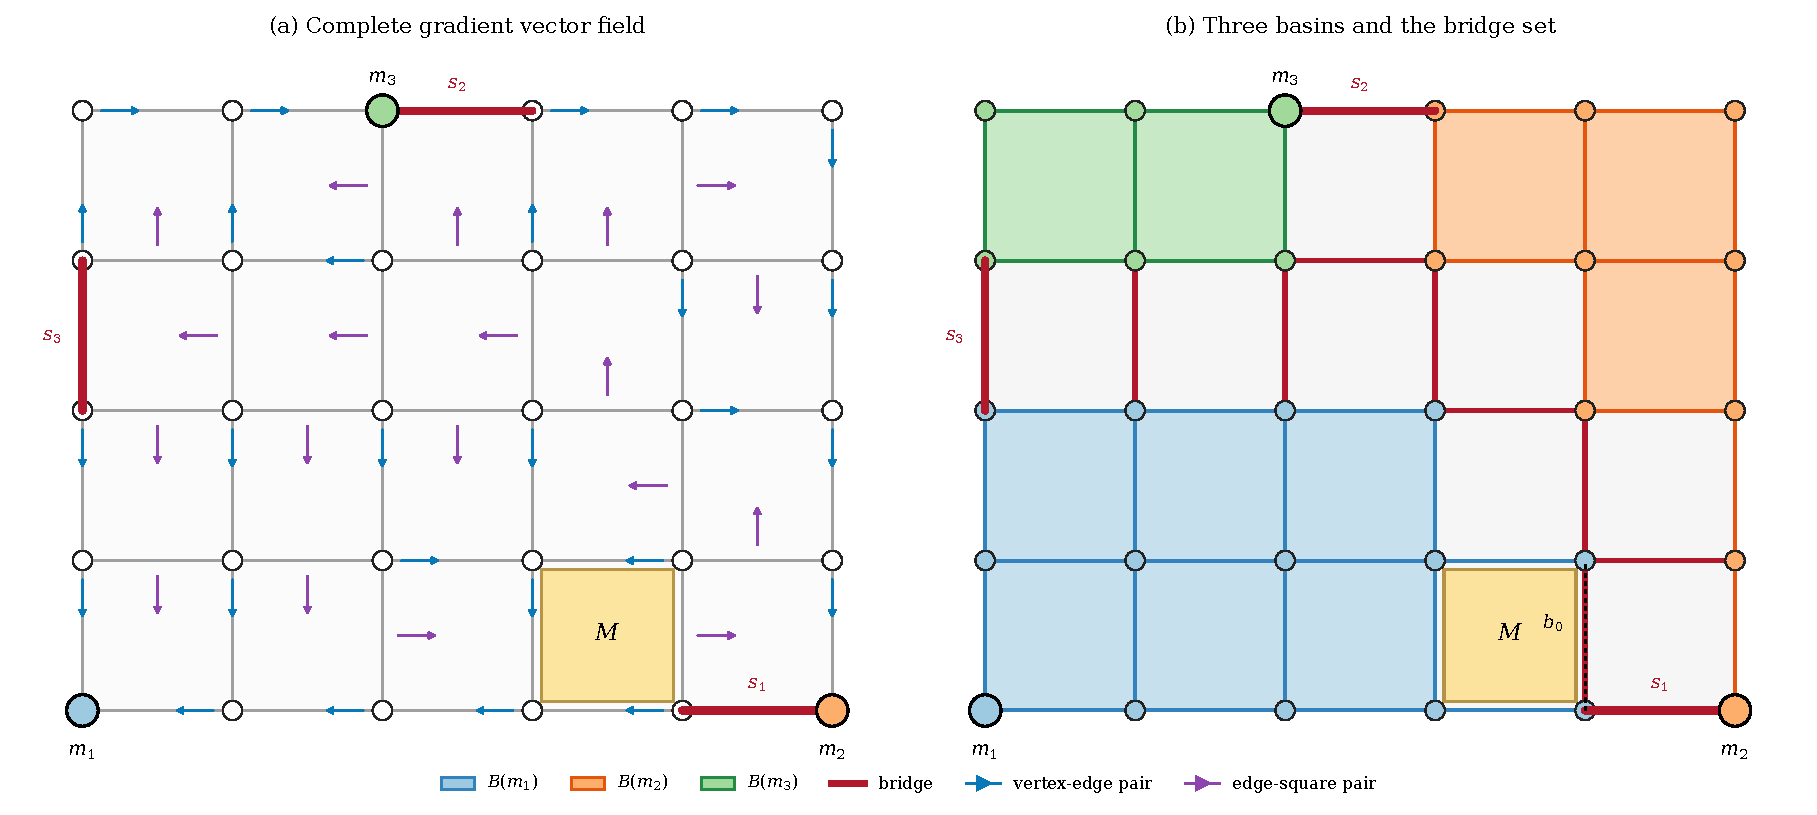
\includegraphics[width=\textwidth]{figures/running_example.pdf}
\caption{A gradient field on a grid of $5\times4$ squares ($99$ cells, $46$
pairs). (a)~Critical cells: three minima $m_1,m_2,m_3$, three saddles
$s_1,s_2,s_3$, one maximum $M$. (b)~The three basins, which are
subcomplexes, and the bridges (red); by Theorem~\ref{thm:bridges} the
bridges form the union of the stable sets of $s_1,s_2,s_3$.}
\label{fig:running}
\end{figure}

% =====================================================================
\section{Order, Flow and Parity}\label{sec:flow}

\begin{lemma}[Order]\label{lem:order}
Let $\kappa_i=(\sigma,\tau)$ be a regular pair of $W$. Then $t(\nu)<i$ for
every $\nu\in\req(\sigma,\tau)$, and $t(\tau')>i$ for every cofacet
$\tau'\ne\tau$ of $\sigma$.
\end{lemma}

\begin{proof}
The cells of $\req(\sigma,\tau)$ are faces of $\sigma$ or $\tau$ distinct
from both, and $K_i=K_{i-1}\cup\{\sigma,\tau\}$ is a complex, so they lie
in $K_{i-1}$. If a cofacet $\tau'\ne\tau$ of $\sigma$ satisfied
$t(\tau')\le i$, then $\tau'\in K_{i-1}$ and, $K_{i-1}$ being closed under
faces, $\sigma\in K_{i-1}$, which is absurd.\qed
\end{proof}

\begin{corollary}\label{cor:decrease}
Insertion steps decrease strictly along gradient paths
($t(\sigma_{i+1})<t(\sigma_i)$) and along cogradient paths
($t(\tau_i)<t(\tau_{i-1})$). In particular $V$ has no closed non-trivial
path.
\end{corollary}

For a critical $p$-cell $\kappa$ we set
$\St(\kappa)=\{\nu\in K^{(p)}:\text{a gradient path joins }\nu\text{ to }\kappa\}$
and
$\Un(\kappa)=\{\nu\in K^{(p)}:\text{a cogradient path joins }\kappa\text{ to }\nu\}$.

\begin{proposition}\label{prop:stable}
For every critical cell $\kappa$:
(i)~$\St(\kappa)=S_K(\kappa)$ and $\Un(\kappa)=U_K(\kappa)$;
(ii)~$\coext(\kappa)\subseteq\St(\kappa)$ and $\ext(\kappa)\subseteq\Un(\kappa)$,
and $\St(\kappa)\setminus\coext(\kappa)$ is the set of cells joined to
$\kappa$ by a positive even number of gradient paths.
\end{proposition}

\begin{proof}
(i) $\St(\kappa)$ contains $\kappa$ and is closed under the rule defining
$S_K(\kappa)$: prefixing $\langle\delta,\gamma\rangle$ to a path from
$\beta\in\partial\gamma$ gives a path from $\delta$. Hence
$S_K(\kappa)\subseteq\St(\kappa)$. Conversely, induction on the length of a
path from $\nu$ to $\kappa$ shows $\nu\in S_K(\kappa)$. The unstable case is
dual. (ii) follows from~\cite[Th.~12]{Ber25a}.\qed
\end{proof}

The inclusions of (ii) are strict as soon as paths branch: on a grid of
$2\times2$ squares with corners $A,\ldots,I$ (row by row), the four pairs
$(AB,ABED)$, $(BE,BCFE)$, $(DE,DEHG)$, $(EF,EFIH)$ give two gradient paths
from $AB$ to the critical edge $EH$, so that $AB\in\St(EH)$ and
$AB\notin\coext(EH)$. Branching is impossible from a vertex.

\begin{theorem}[Vertex flow]\label{thm:flow}
Every vertex $v$ is the origin of a unique maximal gradient path, which ends
at a critical vertex $m(v)$. The number of gradient paths from $v$ to
$m\in\mathcal{M}$ is $1$ if $m=m(v)$ and $0$ otherwise. Consequently
$\St(m)=\coext(m)$ and the sets $\St(m)$, $m\in\mathcal{M}$, partition the
vertices.
\end{theorem}

\begin{proof}
A vertex is never the upper cell of a pair. If $v$ is not critical, the edge
$V(v)$ is unique and has exactly one other vertex, so each step of a path
from $v$ is forced; by Corollary~\ref{cor:decrease} the path terminates, at
an unpaired vertex, i.e.\ a critical one. Every gradient path from $v$ is a
prefix of the maximal one, whose only critical vertex is its endpoint. The
counts follow, and with them the equality with $\coext(m)$ by
Proposition~\ref{prop:stable}.\qed
\end{proof}

This is Lemma~5 of~\cite{DFRS15}, here without any injectivity assumption:
the only properties used are that $V$ is a matching, that an edge has two
vertices, and Corollary~\ref{cor:decrease}.

% =====================================================================
\section{Restriction, Basins and Bridges}\label{sec:basins}

\begin{lemma}\label{lem:hermetic}
Every prefix $K_i$ of $W$ is hermetic. If $W$ is an $F$-sequence for a
stack $F$, every cut $F_\lambda$ is a hermetic subcomplex.
\end{lemma}

\begin{proof}
If $\sigma\in K_i$ and $V(\sigma)=\tau$, both are inserted at step
$t(\sigma)\le i$. A cut is a subcomplex since $F$ is monotone, and
$F(\tau)=F(\sigma)\le\lambda$ when $\sigma\in F_\lambda$.\qed
\end{proof}

\begin{theorem}[Restriction]\label{thm:restriction}
Let $H$ be hermetic and $\kappa\in H$ critical. With the field $V_H$,
$\St_H(\kappa)=\St(\kappa)\cap H$ and $\Un_H(\kappa)=\Un(\kappa)$.
\end{theorem}

\begin{proof}
A path of $V_H$ is a path of $V$. Conversely, a gradient path of $V$
starting in $H$ stays in $H$: if $\sigma_i\in H$ then $\tau_i\in H$ by
hermeticity and $\sigma_{i+1}\in\partial\tau_i\subseteq H$. A cogradient
path starting at $\kappa\in H$ stays in $H$ by the same two
arguments.\qed
\end{proof}

\paragraph{Basins as closures.}
Let $A$ be a subcomplex and $(\sigma,\tau)\in V$ with $\sigma,\tau\notin A$.
The pair is \emph{available} for $A$ if $\req(\sigma,\tau)\subseteq A$; then
$A\cup\{\sigma,\tau\}$ is an elementary expansion of $A$, since a cofacet of
$\sigma$ in $A$ would force $\sigma\in A$. A \emph{basin sequence} rooted at
$m\in\mathcal{M}$ is a chain $\{m\}=B_0\subset B_1\subset\cdots\subset B_r$
where each $B_{j+1}$ adds to $B_j$ a pair available for $B_j$; it is
\emph{maximal} if no pair is available for $B_r$.

\begin{theorem}[Closure]\label{thm:closure}
All maximal basin sequences rooted at $m$ end at the same subcomplex
$B(m)$, and $B(m)$ is the largest subcomplex that collapses regularly onto
$\{m\}$, i.e.\ the basin of~\cite{DFRS15}.
\end{theorem}

\begin{proof}
Let $B$ end a maximal basin sequence. Read backwards, the sequence is a
regular collapse of $B$ onto $\{m\}$, since each added pair is free when
added. Moreover $B$ is $\{m\}$ plus complete pairs of $V$, hence hermetic.
Let $C$ collapse regularly onto $\{m\}$ by removing pairs
$(\sigma_s,\tau_s),\ldots,(\sigma_1,\tau_1)$, and let
$C_j=\{m\}\cup\bigcup_{k\le j}\{\sigma_k,\tau_k\}$. If $C_j\subseteq B$,
then $\req(\sigma_{j+1},\tau_{j+1})\subseteq C_j\subseteq B$ because
$C_{j+1}$ is a complex; by hermeticity the pair is inside or outside $B$,
and outside it would be available, contradicting maximality. Hence
$C\subseteq B$. Two such terminal subcomplexes therefore contain each
other.\qed
\end{proof}

The original proof of uniqueness~\cite[Lem.~6]{DFRS15} compares the values
of an injective function on the cells; here hermeticity and maximality
replace it, and plateaus play no role.

\begin{proposition}\label{prop:basin}
For $m\in\mathcal{M}$: $B(m)$ is hermetic and contractible, $m$ is its only
critical cell, $B(m)^{(0)}=\St(m)$, and basins of distinct minima are
disjoint.
\end{proposition}

\begin{proof}
The first two claims were shown above. If $v\in B(m)$ is a vertex, its
maximal path stays in $B(m)$ by hermeticity and closure, so it ends at $m$.
Conversely, along the path $v=v_0,e_0,v_1,\ldots,v_r=m$ of a vertex of
$\St(m)$, $\req(v_i,e_i)=\{v_{i+1}\}$, so by descending induction and
maximality every $(v_i,e_i)$ lies in $B(m)$. A cell common to two basins
has a vertex common to two stable sets, which Theorem~\ref{thm:flow}
excludes.\qed
\end{proof}

\begin{algorithm}[t]
\caption{All basins in one scan of $W=\langle\kappa_1,\ldots,\kappa_N\rangle$}
\label{alg:basins}
\begin{algorithmic}[1]
\State $\lab(\nu)\gets\bot$ for every cell $\nu$
\For{$i\gets1$ \textbf{to} $N$}
  \If{$\kappa_i$ is a critical vertex}
    $\lab(\kappa_i)\gets\kappa_i$
  \ElsIf{$\kappa_i=(\sigma,\tau)$ and all cells of $\req(\sigma,\tau)$ have
    the same label $m\ne\bot$}
    $\lab(\sigma),\lab(\tau)\gets m$
  \EndIf
\EndFor
\end{algorithmic}
\end{algorithm}

\begin{theorem}\label{thm:algorithm}
Algorithm~\ref{alg:basins} labels $B(m)$ by $m$ for every $m\in\mathcal{M}$
and leaves the other cells at $\bot$, in time
$O(|K|+\sum_{q\in V}|\req(q)|)$, which is $O(d\,|K|)$ in dimension $d$. It
can run while the sequence is produced.
\end{theorem}

\begin{proof}
By Lemma~\ref{lem:order} the labels read at a pair are final. The pairs
labeled $m$, in scan order, form a basin sequence rooted at $m$, which
collapses onto $\{m\}$, so they lie in $B(m)$ by Theorem~\ref{thm:closure}.
Conversely, by induction on the step, a pair of $B(m)$ has its
requirements in $B(m)$, already labeled $m$, so it is labeled $m$; $m$ is
the only critical cell of $B(m)$. Disjointness
(Proposition~\ref{prop:basin}) gives the rest. Each requirement is read
once, and a cubical (resp.\ simplicial) $p$-cell has $2p$ (resp.\ $p+1$)
facets.\qed
\end{proof}

\begin{theorem}[Basins at every level]\label{thm:basin-restriction}
If $H$ is hermetic and $m\in H\cap\mathcal{M}$, the basin of $m$ for $V_H$
is $B(m)\cap H$. In particular, if $W$ is an $F$-sequence, the basins of
every cut $F_\lambda$ and of every prefix are the restrictions of the labels
computed once by Algorithm~\ref{alg:basins}.
\end{theorem}

\begin{proof}
A regular collapse in $H$ is one in $K$, so $B_H(m)\subseteq B(m)\cap H$.
Conversely, intersect a regular collapse of $B(m)$ onto $\{m\}$ with $H$:
each removed pair is inside or outside $H$; outside, nothing changes;
inside, the pair belongs to $V_H$ and stays free. So $B(m)\cap H$
collapses regularly onto $\{m\}$ within $H$. The second claim follows from
Lemma~\ref{lem:hermetic}.\qed
\end{proof}

For a flooding sequence, cuts are prefixes, so the basins of a cut are
those available when the scan of Algorithm~\ref{alg:basins} reaches the
end of the level. No assumption on the injectivity of $F$ is needed.

\begin{theorem}[Bridges]\label{thm:bridges}
Every pair $(v,e)$ of a vertex and an edge lies in a basin, and the set of
bridges is
$\Br=\bigcup\{\St(s): s\text{ critical }1\text{-cell}\}$.
\end{theorem}

\begin{proof}
For $(v,e)\in V$ with other vertex $w$, $\req(v,e)=\{w\}\subseteq B(m(w))$,
so maximality and hermeticity put the pair in $B(m(w))$. If
$e\in\St(s)$, a gradient path from $e$ to $s$ that started in a basin would
stay in it, as in Theorem~\ref{thm:restriction}, and $s$ would be a second
critical cell of that basin; hence $e\in\Br$. Conversely, let $e\in\Br$ be
non-critical. By the first claim, $V(e)=Q$ is a $2$-cell. If every facet of
$Q$ other than $e$ lay in a basin, these facets, which form a connected
path through both vertices of $e$, would lie in a single basin $B(m)$,
since vertices belong to one basin only; then $(e,Q)$ would be available
for $B(m)$. So some $e'\in\partial Q\setminus\{e\}$ is a bridge, and
$\langle e,Q,e'\rangle$ extends a gradient path within $\Br$. By
Corollary~\ref{cor:decrease} the extension stops at a bridge that is
neither paired with a $2$-cell nor, by the first claim, with a vertex: a
critical edge $s$, and $e\in\St(s)$.\qed
\end{proof}

The inclusion ``every bridge is in the stable set of a critical bridge'' is
Lemma~8 of~\cite{DFRS15}; the converse and the proof without a Morse
function are new. Algorithm~\ref{alg:basins} thus also returns the bridges,
as the unlabeled $1$-cells.

% =====================================================================
\section{Simplification and Stacks}\label{sec:simplification}

Let $\alpha$ be a critical $p$-cell and $\beta$ a critical $(p+1)$-cell such
that exactly one gradient path
$\pi=\langle\sigma_0,\tau_0,\ldots,\sigma_r=\alpha\rangle$ starts at a facet
$\sigma_0$ of $\beta$ and ends at $\alpha$. Forman's
\emph{cancellation}~\cite[Sect.~11]{Forman98} replaces the pairs
$(\sigma_i,\tau_i)$ by $(\sigma_{i+1},\tau_i)$ and adds $(\sigma_0,\beta)$;
the result $V'$ is a gradient vector field whose critical cells are those
of $V$ but $\alpha$ and $\beta$. If $V$ is $F$-flat, $V'$ is usually not:
the new pairs join cells of different values.

Components below are connected components in the incidence graph, where a
cell is adjacent to its facets and cofacets. Let $A$ be the component of
$\{\nu:F(\nu)<F(\beta)\}$ containing $\alpha$ ($A=\emptyset$ if
$F(\alpha)=F(\beta)$), and $B$ the component of $\{\nu:F(\nu)>F(\alpha)\}$
containing $\beta$. Define $\Fup=F(\beta)$ on $A$ and $\Fup=F$ elsewhere;
$\Fdown=F(\alpha)$ on $B$ and $\Fdown=F$ elsewhere.

\begin{theorem}[Cancellation and stacks]\label{thm:cancel}
Let $V$ be an $F$-flat gradient vector field and $V'$ obtained by
cancelling $(\alpha,\beta)$. Then $\Fup$ and $\Fdown$ are stacks,
$\Fdown\le F\le\Fup$, and $V'$ is both $\Fup$-flat and $\Fdown$-flat.
Consequently $V'$ is the field of a flooding sequence for $\Fup$ and for
$\Fdown$, and Sections~\ref{sec:flow}--\ref{sec:basins} apply to it at every
level of these stacks.
\end{theorem}

\begin{proof}
Let $c=F(\beta)$. Along $\pi$, faces and flatness give
$c\ge F(\sigma_0)=F(\tau_0)\ge F(\sigma_1)=\cdots\ge F(\alpha)$.

\emph{$\Fup$ is a stack.} Let $\rho\in\partial\nu$. If $\nu\in A$, then
$F(\rho)\le F(\nu)<c$ and $\rho$ is adjacent to $\nu$, so $\rho\in A$. If
$\rho\in A$ and $\nu\notin A$, then $\nu$, adjacent to $\rho$, is not in
$\{F<c\}$, so $\Fup(\nu)=F(\nu)\ge c=\Fup(\rho)$. In the remaining cases
$\Fup$ coincides with $F$ or with $c$ on both cells.

\emph{Old pairs.} A pair $(\sigma,\tau)$ of $V\cap V'$ joins adjacent cells
of equal value, so both or none are in $\{F<c\}$, and both or none in $A$.

\emph{New pairs.} The cells of $\pi$ with $F<c$ form a final segment of
$\pi$, connected and containing $\alpha$, hence contained in $A$; the other
cells of $\pi$ and $\beta$ have value $c$. So $\Fup=c$ on $\beta$ and on
$\pi$, and every new pair is $\Fup$-flat.

The proof for $\Fdown$ is symmetric: the cells of $\pi\cup\{\beta\}$ with
$F>F(\alpha)$ form an initial segment connected to $\beta$, hence lie in
$B$. Finally, an $F'$-flat field $V(W')$ is the field of a flooding
sequence: inserting, among the steps whose requirements are present, one
of smallest value, never gets stuck because $W'$ orders the steps, and
never decreases the value because requirements are faces. This is an
algorithmic form of~\cite[Th.~4.1]{Ber25b}, in $O(N\log N)$.\qed
\end{proof}

For a minimum $m$ and a saddle $s$, $A$ is the connected region below the
level of $s$ around $m$, and $\Fup$ fills it up to that level, which is the
elementary operation of the filtering of minima by
dynamics~\cite{Grimaud92}, known to match persistence~\cite{BNG22,ELZ02}.
Dually, for a saddle and a maximum, $\Fdown$ cuts the maximum down to the
saddle. The stacks differ from $F$ only on one component, so the
simplified field remains readable at every grayscale level.

\begin{proposition}[Merging]\label{prop:merge}
Let $s$ be a critical edge with vertices $a,b$ such that $m(a)=m\ne m(b)=m'$.
Then $(m,s)$ can be cancelled; denote by $B'$ the basins of the result.
Then $B'(m')\supseteq B(m)\cup B(m')\cup\{s\}$, the vertex sets satisfy
$B'(m')^{(0)}=B(m)^{(0)}\cup B(m')^{(0)}$, and $B'(m'')=B(m'')$ for every
other $m''\in\mathcal{M}$.
\end{proposition}

\begin{proof}
By Theorem~\ref{thm:flow}, exactly one gradient path goes from $a$ to $m$
and none from $b$. It consists of vertices of $\St(m)$ and of the edges
paired with them, which lie in $B(m)$. A basin sequence of $B(m'')$ for $V$
remains one for $V'$, and no pair of $V'$ becomes available for it: the
reversed pairs require a vertex of $\St(m)$, and $(a,s)$ requires $b\in
B(m')$. So $B'(m'')=B(m'')$ by Theorem~\ref{thm:closure}. A basin sequence
of $B(m')$ continues with $(a,s)$, then with the reversed pairs of $\pi$
down to $m$, and then with the pairs of a basin sequence of $B(m)$. The
vertex flows of $\St(m)$ now reach $a$, then $s$, then $m'$.\qed
\end{proof}

The inclusion can be strict: a pair whose requirements met both $B(m)$ and
$B(m')$ becomes available. Iterating cancellations of minimum--saddle pairs
of persistence below a threshold, each followed by the update $\Fup$, keeps
an $F$-flat field at every step; Section~\ref{sec:experiments} illustrates
it.

% =====================================================================
\section{From Grayscale Images}\label{sec:lowerstars}

Let $f$ be a vertex map and $\prec$ the total order on vertices given by
$f$, ties being broken by a fixed order. The \emph{lower star} $L(x)$ of a
vertex $x$ is the set of cells whose $\prec$-largest vertex is $x$; lower
stars partition $K$ and the max-extension $F$ is constant on each.
Algorithm~1 of RWS~\cite{RWS11} processes each $L(x)$ independently: if
$L(x)\ne\{x\}$, it pairs $x$ with its smallest edge for the lexicographic
order on decreasing vertex values, then repeatedly pairs a queued cell
having exactly one unclassified face in $L(x)$ with that face, and declares
critical a queued cell with none. The resulting field is $F$-flat, since
pairs stay in one lower star, so the scheduling used in the proof of
Theorem~\ref{thm:cancel} turns it into a flooding sequence. Bertrand and Najman state that the core
of this algorithm and of their lower-star algorithm are the same~\cite{BN25};
the following makes precise the variant implemented in \morseq.

\begin{proposition}\label{prop:rws}
On cubical and simplicial complexes, Algorithm~1 of~\cite{RWS11} returns
the same field if (i)~ties are broken by a vertex order instead of a ramp
added to $f$, (ii)~unclassified \emph{facets} are counted instead of faces,
(iii)~the lower star is rescanned after each classification instead of
visiting the cofaces of the classified cells, and (iv)~classified cells are
skipped when dequeued instead of removed from the queue.
\end{proposition}

\begin{proof}
(i) yields the same total order. For (ii), each classified cell of $L(x)$
has all its faces in $L(x)$ classified: this holds for $x$ and its edge,
and is preserved since a cell is paired only with its unique unclassified
face and made critical only without one. Let $\nu\in L(x)$ be unclassified
and $\beta$ an unclassified face of $\nu$ of codimension $k\ge2$. The
interval $[\beta,\nu]$ is a Boolean lattice and contains $k$ facets of
$\nu$; each contains $x$, lies in $L(x)$, and has the unclassified face
$\beta$, so it is unclassified. Hence $\nu$ has no, exactly one, or at least
two unclassified faces exactly when it has no, exactly one, or at least two
unclassified facets, and a unique unclassified face is a facet. For (iii),
when $x$ and its edge $\delta$ are classified, a cell of $L(x)$ that does
not contain $\delta$ has no unclassified face if it is an edge and at least
two (two edges through $x$) otherwise, so the cells with exactly one are
cofaces of $\delta$, as queued by RWS; afterwards only the cofaces of a
newly classified cell can change their count. The queue thus receives the
same cells, and since cells are compared by distinct words, the same cells
are dequeued. (iv) changes nothing to the output.\qed
\end{proof}

% =====================================================================
\section{Experiments}\label{sec:experiments}

\morseq is written in pure Python, for cubical complexes of any dimension
and simplicial complexes. Every statement above is a test, and every number
below is produced by a script of the repository (folder
\texttt{paper/experiments}).

\paragraph{Systematic checks.}
On \nRWSimages{} random images with plateaus, in 2-D and 3-D
(\nRWScells{} cells in total), the field of \morseq and a line-by-line
transcription of RWS Algorithm~1 coincide (\nRWSdiff{} differences). On
\nCancelStacks{} stacks, all \nCancelPairs{} cancellable pairs were cancelled:
$V'$ was not $F$-flat in \nCancelNotFlat{} cases (\nCancelNotFlatPct\,\%);
it was $\Fup$-flat and
$\Fdown$-flat in all cases, and the schedule of Theorem~\ref{thm:cancel}
produced a flooding sequence for $\Fup$ each time (the test suite also
checks it for $\Fdown$ on a smaller set).
Proposition~\ref{prop:merge} held for all \nMerges{} minimum--saddle
cancellations. On \nSeqs{} random Morse sequences and image sequences
(\nSeqCells{} cells), Algorithm~\ref{alg:basins} agreed with the closure of
Theorem~\ref{thm:closure} and Theorem~\ref{thm:bridges} held in all cases,
and existence was strictly larger than parity in \nStrict{} of them.

\paragraph{Running time.}
Table~\ref{tab:runtime} reports the three stages on random 8-bit images
(\runtimeMachine), up to \runtimeMaxCells{} cells. The total time per cell
stays between \runtimeMinUs{} and \runtimeMaxUs~$\mu$s and does not grow with
the size, as expected from Theorem~\ref{thm:algorithm} and the
$O(N\log N)$ schedule; the variations come from the load of the machine.
Basin labeling is the cheapest stage.

\begin{table}[t]
\centering
\caption{Running time of the stages: lower-star gradient, flooding
sequence, basin labeling (pure Python, best of two runs, each size in a
separate process).}
\label{tab:runtime}
\small
\begin{tabular}{@{}lrrrrrr@{}}
\toprule
grid & cells & minima & gradient & sequence & basins & $\mu$s/cell \\
\midrule
$64\times64$ & 16\,129 & 853 & 0.4\,s & 0.3\,s & 0.0\,s & 44 \\
$128\times128$ & 65\,025 & 3\,240 & 1.8\,s & 1.4\,s & 0.2\,s & 52 \\
$256\times256$ & 261\,121 & 13\,003 & 11.6\,s & 5.3\,s & 0.8\,s & 68 \\
$512\times512$ & 1\,046\,529 & 52\,547 & 25.5\,s & 24.0\,s & 2.9\,s & 50 \\
$16\times16\times16$ & 29\,791 & 598 & 2.1\,s & 0.9\,s & 0.2\,s & 109 \\
$24\times24\times24$ & 103\,823 & 2\,060 & 8.3\,s & 3.6\,s & 0.7\,s & 121 \\
$32\times32\times32$ & 250\,047 & 4\,807 & 8.9\,s & 4.3\,s & 0.9\,s & 56 \\
\bottomrule
\end{tabular}

\end{table}

\paragraph{Simplification.}
Figure~\ref{fig:simplification} shows an 8-bit $\simplN\times\simplN$
image made of \simplWells{} Gaussian wells and uniform noise of amplitude
$\pm\simplNoise$. Its lower-star field has \simplMinStart{} critical
vertices. We cancel minimum--saddle pairs whose persistence
$F(s)-F(m)$ is below a threshold $h$, lowest first, each cancellation being
followed by the update $\Fup$. The minima left are exactly the
\simplWells{} wells for $\simplPlateauLo\le h\le\simplPlateauHi$; beyond,
wells start to merge, and \simplMinEnd{} minima remain for $h=\simplHEnd$
(\simplCancel{} cancellations in total). After every
cancellation the field is flat for the current stack, which never
decreases, so that the basins of the simplified field are given at every
level by Algorithm~\ref{alg:basins}.

\begin{figure}[t]
\centering
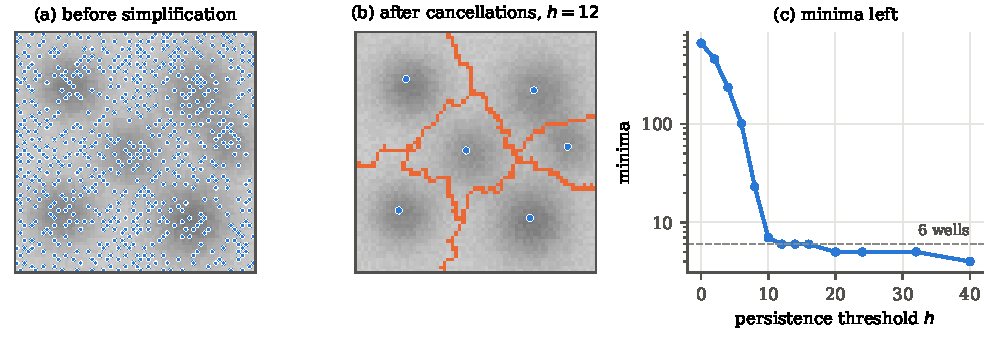
\includegraphics[width=\textwidth]{figures/simplification.pdf}
\caption{Simplification of a noisy image. (a)~The image and its
\simplMinStart{} minima (blue). (b)~The minima left after cancelling all
minimum--saddle pairs of persistence below $h=\simplHShow$, and the
boundaries between their vertex classes (orange). (c)~Number of minima left
as a function of $h$ (logarithmic scale); the dashed line marks the
\simplWells{} wells.}
\label{fig:simplification}
\end{figure}

% =====================================================================
\section{Conclusion}

The segmentation layer of discrete Morse theory translates to Morse
sequences with short proofs: the insertion order replaces the injective
function, hermeticity replaces comparisons of values, and plateaus need no
special treatment. The same order schedules the computation of all basins
in one scan. Cancellation, which leaves the $F$-sequence framework, comes
back into it through an explicit modification of the stack on a single
component.

Three questions remain. The Morse skeleton and the regular collapse of a
complex onto it~\cite{DFRS15} should follow from the same tools applied to
unstable sets. The stacks $\Fup$ and $\Fdown$ are explicit but not claimed
minimal; characterizing the smallest stack above $F$ for which $V'$ is flat
is open. Finally, iterated minimum--saddle cancellation with $\Fup$ should
be compared with the watershed of the image filtered by
dynamics~\cite{Grimaud92,NS96}, whose equivalence with persistence is
known~\cite{BNG22}.

\paragraph{Acknowledgements.}
This work originated in a research internship at the Laboratoire
d'Informatique Gaspard-Monge (LIGM).

\paragraph{Disclosure.}
The software and the manuscript were prepared with the assistance of a
large language model (Claude, Anthropic). The author is responsible for
the content; every statement is accompanied by an executable test in the
public repository.

\bibliographystyle{splncs04}
\bibliography{references}

\end{document}
